\documentclass{article}

\usepackage{graphicx}
\usepackage{tikz}
\usepackage{tikzsymbols}
\usetikzlibrary{calc,patterns,shapes.geometric}
\pagestyle{empty}
\usepackage[margin=0pt]{geometry}
\geometry{papersize={14in,12in}}

\def\centerarc[#1](#2)(#3:#4:#5){\draw[#1] ($(#2)+({#5*cos(#3)},{#5*sin(#3)})$) arc (#3:#4:#5);}

\begin{document}
	\begin{figure}
		\centering
		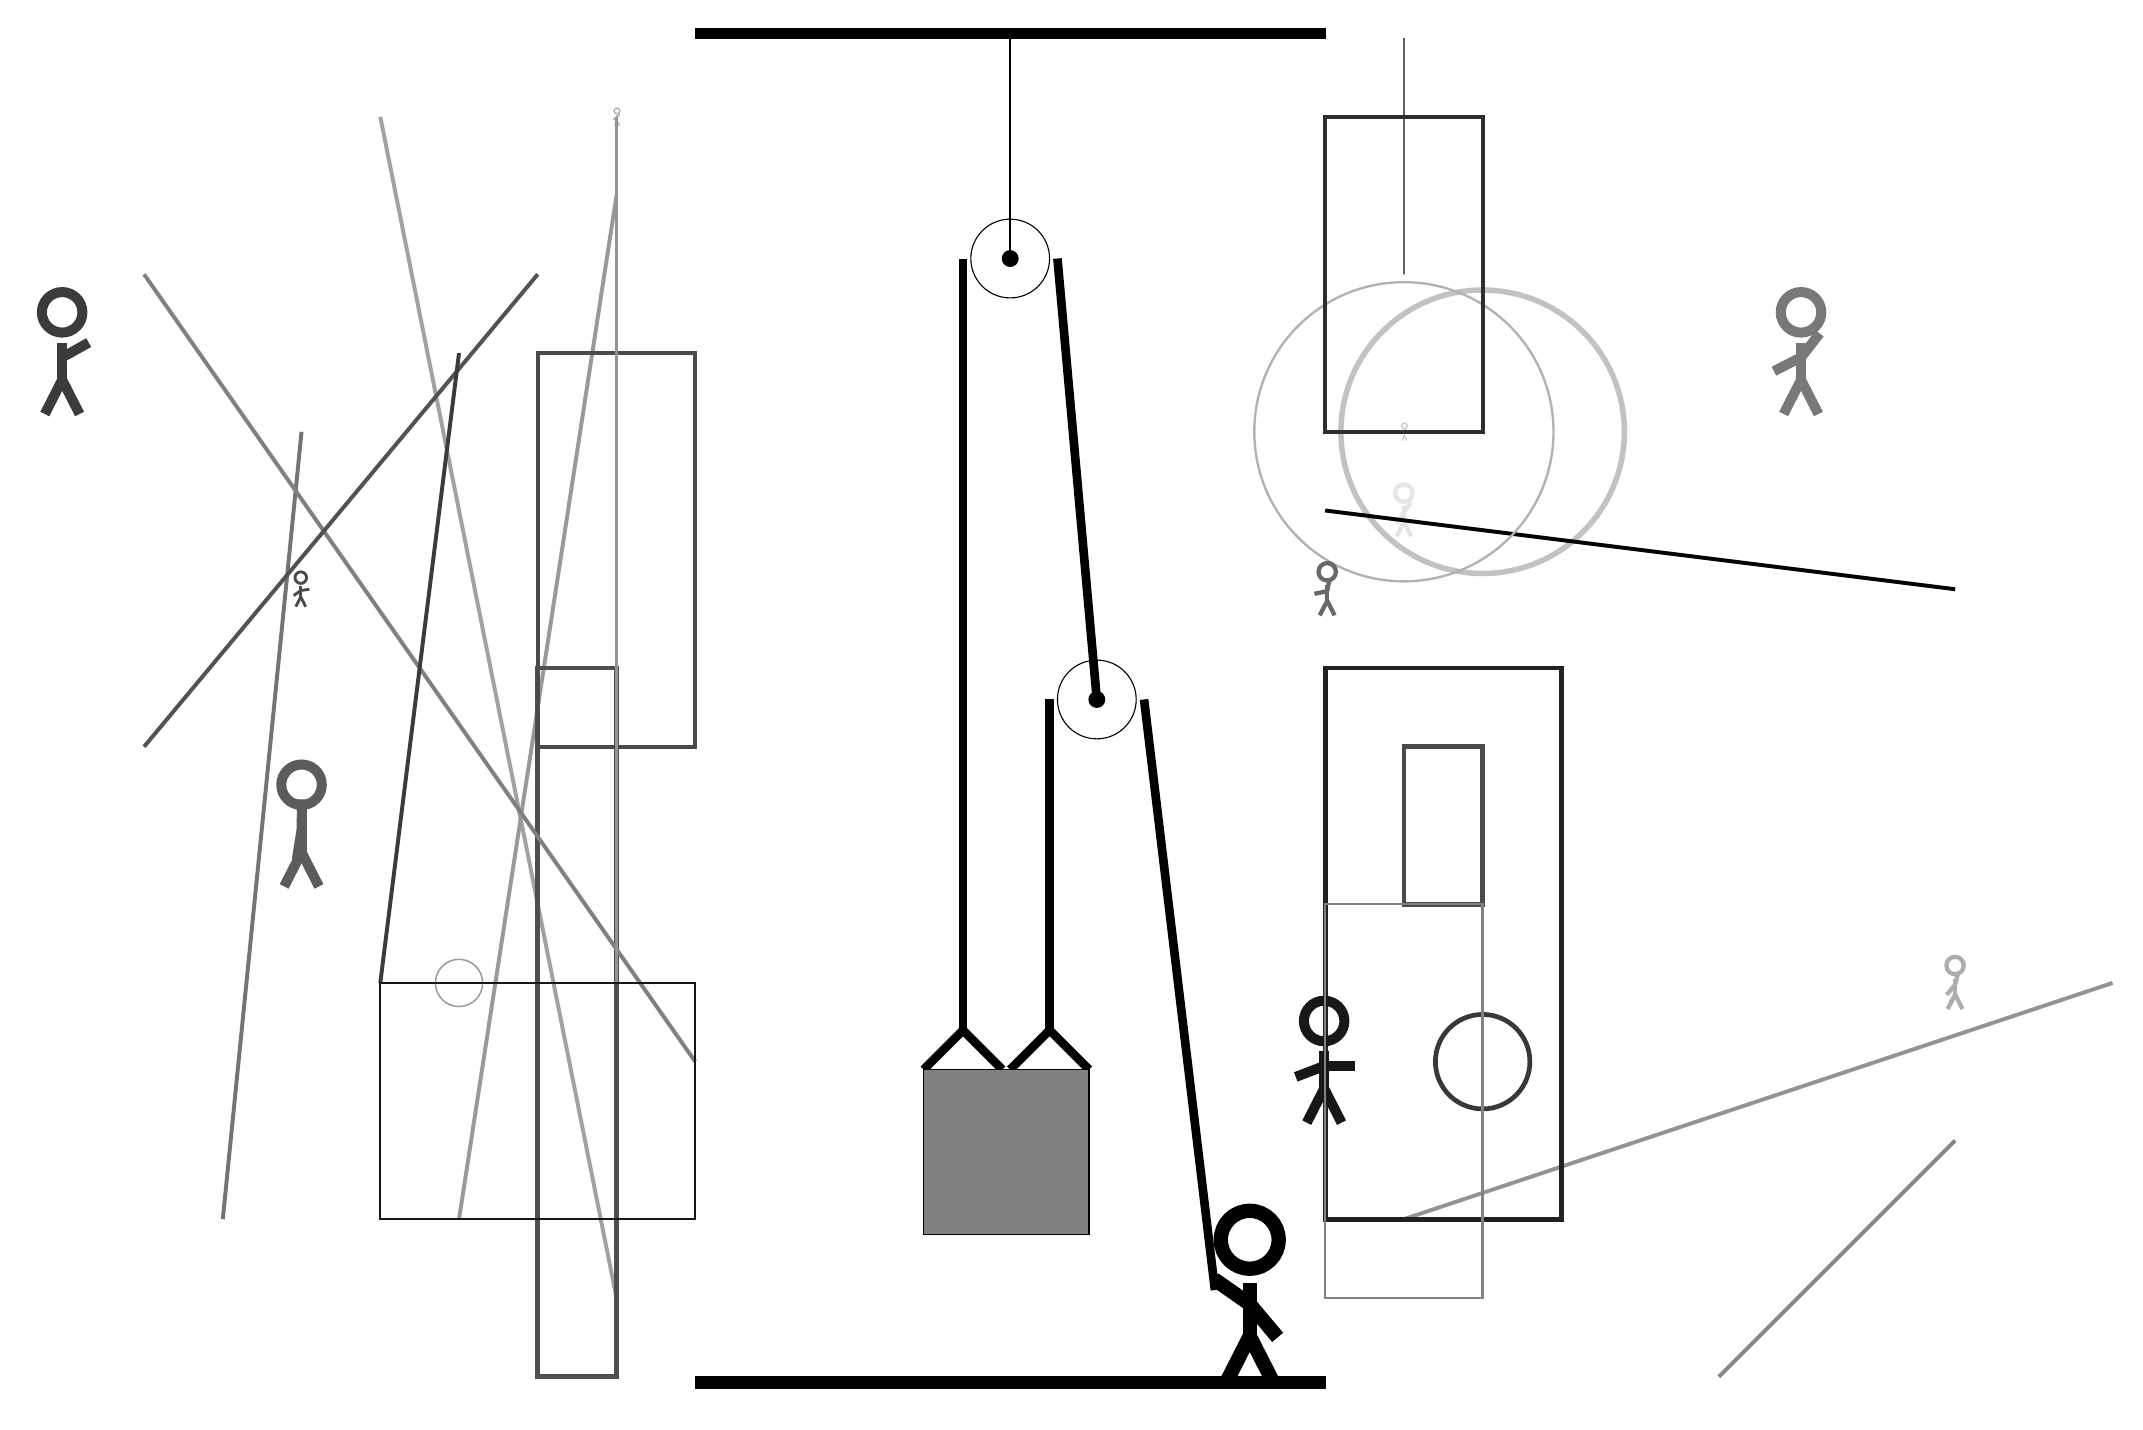
\begin{tikzpicture}
			%%%%% START %%%%%
			
			\draw[fill=black] (-2, 14) rectangle (6, 14.125);
			
			\draw (2, 11.2) circle (0.5);
			\draw[fill=black] (2, 11.2) circle (0.1);
			\draw[thick] (2, 11.2) -- (2, 14);
			
			\draw (3.1, 5.6) circle (0.5);
			\draw[fill=black] (3.1, 5.6) circle (0.1);
			
			\draw[line width = 1.1mm]  (0.9, 0.9) -- (1.4, 1.4) -- (1.9, 0.9);
			\draw[line width = 1.1mm]  (2.0, 0.9) -- (2.5, 1.4) -- (3.0, 0.9);
			\draw[fill=black!50] (0.9, 0.9) rectangle (3.0, -1.2);
			
			\draw[line width = 1.1mm] (1.4, 11.2) -- (1.4, 1.4);
			\centerarc[line width = 1.1mm](2, 11.2)(0:180:0.6);
			\draw[line width = 1.1mm] (2.6, 11.2) -- (3.1, 5.6);
			\draw[line width = 1.1mm] (2.5, 5.6) -- (2.5, 1.4);
			\centerarc[line width = 1.1mm](3.1, 5.6)(0:180:0.6);
			\draw[line width = 1.1mm] (3.7, 5.6) -- (4.6, -1.9);
			
			\draw[line width=0.5mm, color=black!42](7, -1) -- (16, 2);
			
			\draw [line width=0.7mm, color=black!24](8, 9) circle (1.8);
			\draw[line width=0.5mm, color=black!37](-6, 13) -- (-3, -2);
			\node[line width=0.4mm, color=black!30] at (-3, 13) {\Strichmaxerl[1][23][48]};
			\draw[line width=0.6mm, color=black!71] (7, 3) rectangle (8, 5);
			\draw[line width=0.5mm, color=black!40](-5, -1) -- (-3, 12);
			
			\node[line width=0.6mm, color=black!77] at (-10, 10) {\Strichmaxerl[7][90][29]};
			\draw[line width=0.6mm, color=black!87] (6, 6) rectangle (9, -1);
			\draw [line width=0.6mm, color=black!78](8, 1) circle (0.6);
			\draw[line width=0.5mm, color=black!47](11, -3) -- (14, 0);
			\node[line width=0.5mm, color=black!10] at (7, 8) {\Strichmaxerl[3][55][56]};
			
			\draw[line width=0.4mm, color=black!42] (-2, -2) rectangle (-2, -2);
			\node[line width=0.4mm, color=black!53] at (12, 10) {\Strichmaxerl[7][27][52]};
			\draw[line width=0.5mm, color=black!55](-7, 9) -- (-8, -1);
			\draw[line width=0.6mm, color=black!69] (-4, -3) rectangle (-3, 6);
			\draw[line width=0.5mm, color=black!99](6, 8) -- (14, 7);
			
			\node[line width=0.5mm, color=black!20] at (7, 9) {\Strichmaxerl[1][22][70]};
			\draw [line width=0.2mm, color=black!38](-5, 2) circle (0.3);
			\draw [line width=0.3mm, color=black!30](7, 9) circle (1.9);
			\draw[line width=0.5mm, color=black!71] (-2, 10) rectangle (-4, 5);
			\draw[line width=0.2mm, color=black!61] (7, 11) rectangle (7, 14);
			
			\draw[line width=0.5mm, color=black!50](-2, 1) -- (-9, 11);
			\draw[line width=0.5mm, color=black!82] (6, 13) rectangle (8, 9);
			\draw[line width=0.5mm, color=black!68](-4, 11) -- (-9, 5);
			\node[line width=0.4mm, color=black!64] at (-7, 4) {\Strichmaxerl[7][81][89]};
			
			\draw [line width=0.6mm, color=black!25](8, 11) circle (0.0);
			\draw[line width=0.5mm, color=black!58](11, 9) -- (11, 9);
			\node[line width=0.4mm, color=black!59] at (6, 7) {\Strichmaxerl[3][12][79]};
			
			\node[line width=0.6mm, color=black!71] at (-7, 7) {\Strichmaxerl[2][36][8]};
			\node[line width=0.6mm, color=black!32] at (14, 2) {\Strichmaxerl[3][50][76]};
			\draw[line width=0.5mm, color=black!42] (-3, 2) rectangle (-3, 13);
			
			\node[line width=0.7mm, color=black!91] at (6, 1) {\Strichmaxerl[7][21][0]};
			\draw[line width=0.5mm, color=black!77](-5, 10) -- (-6, 2);
			
			\draw[line width=0.3mm, color=black!91] (-2, -1) rectangle (-6, 2);
			
			\draw[line width=0.3mm, color=black!49] (8, -2) rectangle (6, 3);
			
			\node at (5, -2) {\Strichmaxerl[10][-35][-50]};
			
			\draw[fill=black] (-2, -3) rectangle (6, -3.15);
			
			%%%%% END %%%%%
		\end{tikzpicture}
	\end{figure}	
\end{document}